%==============================================================================
% Sjabloon poster bachproef
%==============================================================================
% Gebaseerd op document class `a0poster' door Gerlinde Kettl en Matthias Weiser
% Aangepast voor gebruik aan HOGENT door Jens Buysse en Bert Van Vreckem

\documentclass[a0,portrait]{hogent-poster}

% Info over de opleiding
\course{Bachelorproef}
\studyprogramme{toegepaste informatica}
\academicyear{2025-2026}
\institution{Hogeschool Gent, Valentin Vaerwyckweg 1, 9000 Gent}

% Info over de bachelorproef
\title{Van reactief naar proactief: een centraal observability-platform voor multi-site live-streaming}
\subtitle{Een proof-of-concept voor metrics-, log- en flowmonitoring binnen Mediaventures}
\author{Emiel Vandenberghe}
\email{emiel.vandenberghe@student.hogent.be} % TODO: controleer je exacte student-e-mail
\supervisor{M. Saelens (HOGENT)}
\cosupervisor{A. Van Renterghem (Mediaventures)}

% Indien ingevuld, wordt deze informatie toegevoegd aan het einde van de
% abstract. Zet in commentaar als je dit niet wilt.
\specialisation{Systeem- en Netwerkbeheer} % TODO: controleer je afstudeerrichting
\keywords{Observability, Monitoring, PLG-stack, SRT, NDI, PepVPN}
\projectrepo{https://github.com/EmielVandenberghe/bachp-mediaventures}

\begin{document}

\maketitle

\begin{abstract}
Mediaventures verzorgt livestreaming voor internationale medische congressen, waarbij meerdere live-surgery-locaties en venues realtime video en audio uitwisselen. De bestaande monitoring is lokaal en gefragmenteerd: er is geen end-to-end zicht op de keten, waardoor techniekers bij storingen handmatig op elk toestel moeten inloggen. Deze bachelorproef ontwerpt en bouwt een gecentraliseerd observability-platform op basis van de open-source PLG-stack (Prometheus, Loki, Grafana) met custom Python-exporters. Het platform verzamelt meer dan 40 metrics uit vijf onafhankelijke bronnen en maakt netwerk-, transport-, applicatie- en AV-hardwarelaag gelijktijdig zichtbaar in \'e\'en dashboard, met actieve alerting naar Microsoft Teams. De kernbijdrage is de verschuiving van reactieve, kwalitatieve detectie tijdens korte testsessies naar continue, geautomatiseerde 24/7-meting.
\end{abstract}

\begin{multicols}{2} % This is how many columns your poster will be broken into, a portrait poster is generally split into 2 columns

\section{Introductie}

Tijdens live-surgeryprojecten verbindt Mediaventures meerdere geografisch gescheiden locaties die gelijktijdig video en audio uitwisselen over een complexe keten van routers, 5G- en satellietverbindingen, NDI-netwerken en SRT-encoders. Een probleem op \'e\'en plaats werkt meteen door op meerdere locaties.

De huidige monitoring is echter \emph{lokaal en gefragmenteerd}: elke locatie bewaakt enkel de eigen omgeving en er is geen zicht op de inter-site verbindingen. Bij storingen moeten techniekers handmatig op elk apparaat inloggen, wat traag is en het risico op kwaliteitsverlies vergroot. Bovendien zijn er vandaag geen gemeten referentiewaarden: v\'o\'or elke uitzending controleren techniekers de keten ongeveer dertig minuten handmatig en op het oog, zonder cijfers die vastleggen wat een normale verbinding is. Afwijkingen worden zo pas laat en op gevoel opgemerkt.

\textbf{Onderzoeksvraag:} Hoe kan Mediaventures een ge\"integreerde observability-oplossing inzetten om de volledige audiovisuele infrastructuur end-to-end op te volgen en storingen sneller te detecteren?

\section{Experimenten}

De oplossing werd ontwikkeld en gevalideerd in een volledig virtuele testomgeving: vier FusionHub-routers en \'e\'en fysieke Peplink Balance~20X, verbonden via een VyOS-router. Netwerkstoringen werden gecontroleerd nagebootst om de detectie te testen. De observability-stack draait als veertien Docker-containers op \'e\'en host.

Negen testscenario's dekken samen de volledige keten af: storingen op de netwerklaag (vertraging, pakketverlies, uitval), op de streamlaag (SRT en NDI), op de fysieke hardware, en de end-to-end alerting naar Microsoft~Teams. In elk scenario werd de storing binnen \'e\'en tot vijf minuten gedetecteerd en gevisualiseerd.

Twee inzichten kwamen sterk naar voren. Het combineren van meerdere onafhankelijke databronnen voorkomt valse meldingen, doordat de bronnen elkaar controleren. En een zelf-gevonden fout in de stack, waarbij alle tunnels als actief werden gemeld terwijl er geen geconfigureerd waren, toonde dat een monitoringsysteem ``geen data'' nooit als ``alles in orde'' mag interpreteren.

\section{Architectuur}

Custom Python-exporters vertalen de InControl2-API, SNMP, de lokale Peplink-API en de SRT-, NDI- en BirdDog-bronnen naar het Prometheus-formaat. Prometheus en Loki slaan respectievelijk metrics en logs op; Grafana visualiseert en alarmeert.

\begin{center}
  \captionsetup{type=figure}
  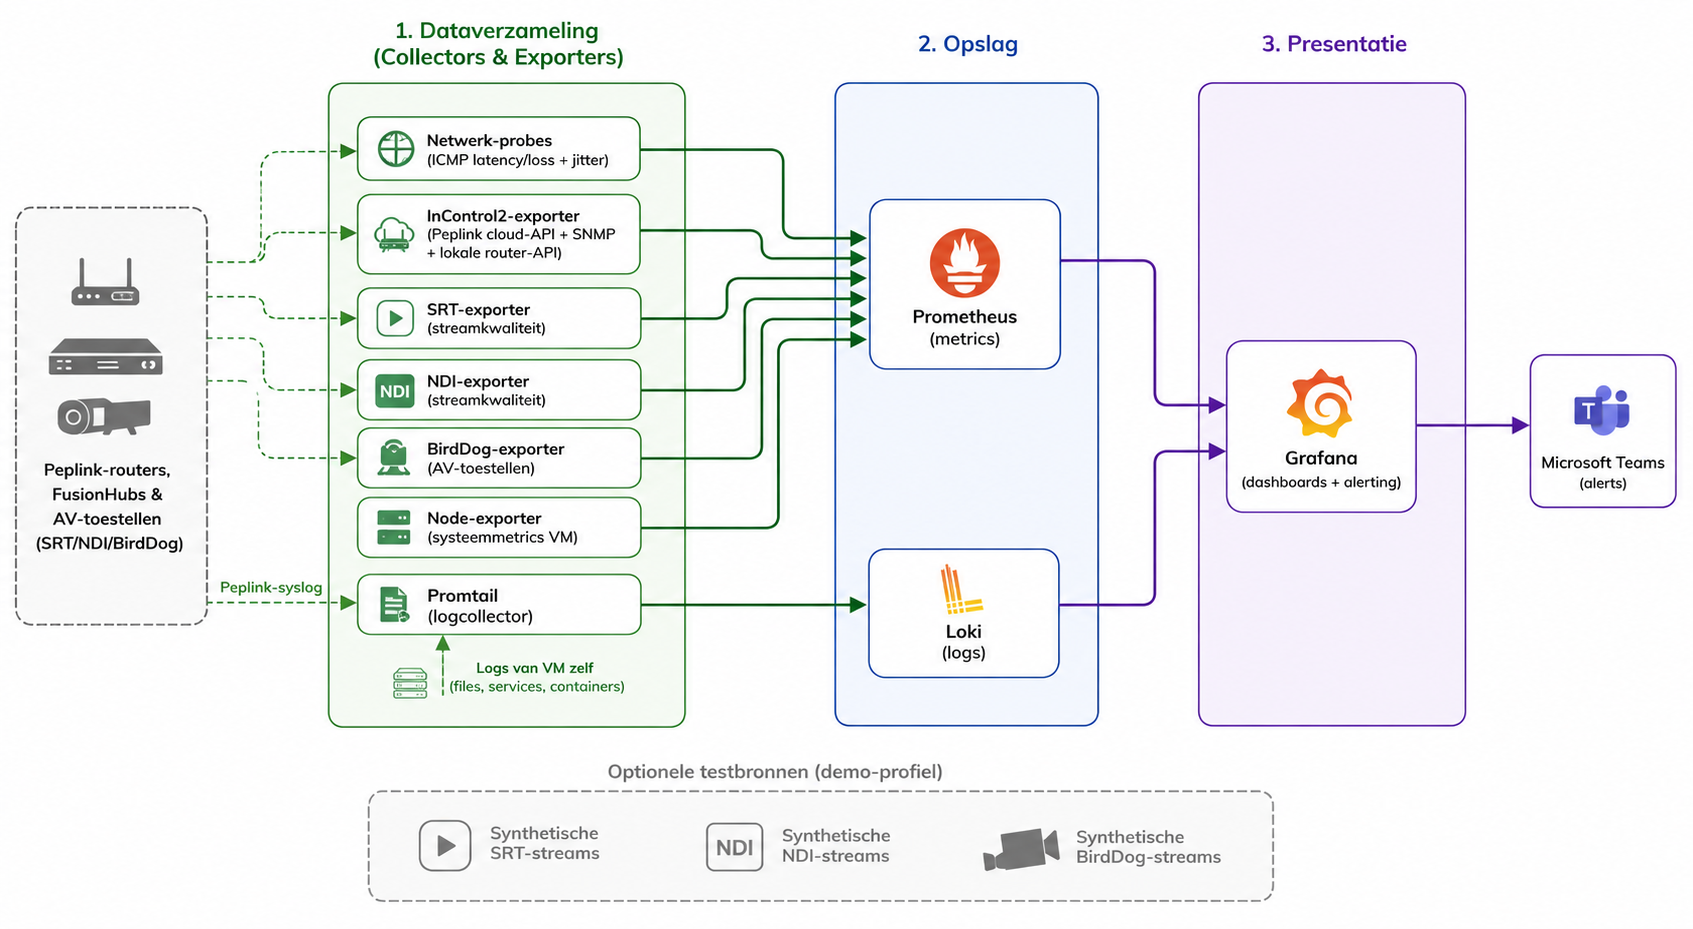
\includegraphics[width=1.0\linewidth]{architectuur}
  \captionof{figure}{De observability-architectuur in drie lagen: collectors en exporters (laag~1) verzamelen metrics en logs uit de Peplink-, stream- en AV-bronnen; Prometheus en Loki slaan ze op (laag~2); Grafana visualiseert en alarmeert richting Microsoft Teams (laag~3).}
\end{center}

\section{Conclusies}

Een open-source PLG-stack met custom exporters kan de volledige audiovisuele keten van Mediaventures end-to-end bewaken. Realistische storingen op netwerk-, device-, applicatie- en AV-hardwarelaag worden binnen 1 tot 5~minuten gedetecteerd, gevisualiseerd en actief gemeld aan het NOC via Microsoft Teams.

De winst zit niet in een gemeten tijdsverschil, want zo'n baseline bestond niet. Ze zit in de overstap van handmatig controleren tijdens een korte testsessie per project naar \textbf{continue, geautomatiseerde 24/7-meting}. Even belangrijk is de \emph{houding} die mee wordt overgedragen: elk metric wantrouwen, elke aanname benoemen en elke blinde vlek openlijk rapporteren. Het resultaat is een overdraagbaar prototype dat met enkel configuratie en een aanvullende security-review naar productie kan doorgroeien.

\section{Toekomstig onderzoek}

\begin{itemize}
  \item De NDI-exporter is getest met een softwarematige testbron. Valideren tegen echte hardware-encoders en bronnen over meerdere VLAN's (via een NDI Discovery Server) moet bevestigen dat de metingen ook in productie kloppen.
  \item Storingen worden nu visueel gecorreleerd door een operator. Automatische correlatie, eerst met regels en later eventueel machine learning, kan samenhangende alarmen zelf bundelen tot \'e\'en vermoedelijke oorzaak.
  \item Het dashboard dekt routers en streams, maar nog geen switches (Netgear M4250) of audio-mengtafels. Die toevoegen maakt de keten pas echt volledig.
  \item De stack meet streamstatistieken zoals bitrate en packet loss, niet de zichtbare beeldkwaliteit. Perceptuele metrieken (PSNR/SSIM) op decoder-niveau zouden meten wat de kijker effectief ziet.
\end{itemize}

\end{multicols}
\end{document}
